%%%%%%%%%%%%%%%%%%%%%%%%%%%%%%%%%%%%%%%%%%%%%%%%%%%%%%%%%%%%%%%%%%%%%%%%%%%%%%%%
% \documentclass[12pt,papel,twoside]{ibtesis}
% \documentclass[12pt,papel,singlespace,oneside]{ibtesis}
% \documentclass[12pt,papel,preprint,singlespace,oneside]{ibtesis}

\documentclass[screen,pagebackref]{ibtesis}
% Antes acá estaba
% \documentclass[12pt,screen,twoside,pagebackref]{ibtesis}


%%%%%%%%%%%%%%%%%%%%% Paquetes extra %%%%%%%%%%%%%%%%%%%%%%%%%%%%%%%%%%%%%%%%%%%
% Por conveniencia: aqu\'{\i} puede cargar todos los paquetes y definir los comandos 
% que necesite
\usepackage{ibextra}
\usepackage{xurl}
\usepackage{caption}
\usepackage{subcaption}
\usepackage{amssymb} 
\usepackage{cancel}
\usepackage[dvipsnames]{xcolor}
\usepackage{listings}
\usepackage{graphicx}
\usepackage{wrapfig}
\usepackage{lscape}
\usepackage{rotating}
\usepackage{epstopdf}
\newcommand{\grad}{^{\circ}}
%\usepackage{hyphen-spanis}
%%%%%%%%%%%%%%%%%%%%%%%%%%%%%%%%%%%%%%%%%%%%%%%%%%%%%%%%%%%%%%%%%%%%%%%%%%%%%%%%
%%%%%%%%%%%%%%%%%%%%% Informacion sobre la tesis %%%%%%%%%%%%%%%%%%%%%%%%%%%%%%%
\title{Conformación digital de haz para recepción de señales satelitales}
\author{Lucas Mariano Grigolato}
\director{Dr. Santiago Hernandez}
\codirector{Ing. Nicolás Catalano}
\carrera{Proyecto Integrador de la Carrera de Ingeniería en Telecomunicaciones}
\grado{Estudiante}
\laboratorio{Departamento de Ingeniería en Telecomunicaciones\\Comisión Nacional de Energía Atómica\\Centro Atómico Bariloche}
\jurado{Ing. Roberto Costantini (INVAP - Instituto Balseiro)\\ 
Dr. Damián Dellavale Clara (CONICET - Instituto Balseiro)}
\palabrasclave{Instituto Balseiro,Conformación de haz, arreglo de antenas en fase, ESPRIT, MUSIC, Muestreo Aleatorio, Aprendizaje Automático, Máquina de Vectores de Soporte, GNU Radio, FPGA}
\keywords{Instituto Balseiro, Beamforming, Phased array antenna, ESPRIT, MUSIC, Random Sampling, Machine Learning, Support vector machine, GNU Radio, FPGA}
% Si queremos poner la fecha manualmente:
\date{17 de Diciembre de 2020}

%%%%%%%%%%%%%%%%%%%%%%%%%%%%%%%%%%%%%%%%%%%%%%%%%%%%%%%%%%%%%%%%%%%%%%%%%%%%%%%%
%\titlepagefalse % Si no quiere compilar la portada descomente esta linea
%\includeonly{apendices} % Compilar s\'{o}lo estos archivos 
\graphicspath{{figs/}} % Lugar donde encontrar las figuras generales (se puede poner uno en cada cap{\'{\i}}tulo)
%%%%%%%%%%%%%%%%%%%%%%%%%%%%%%%%%%%%%%%%%%%%%%%%%%%%%%%%%%%%%%%%%%%%%%%%%%%%%%%%


\begin{document}

% Dentro del environment 'preliminary' va:
% la dedicatoria, resumen, abstract, indices

\begin{preliminary}

    % Escriba su dedicatoria
    \dedicatoria{
        A mi mamá\\
        y a mis hermanos Fer y Palito,\\
        máximos responsables de que haya podido llegar hasta acá.
    }

    %%% \'{I}ndices %%%%

    \begin{abreviaturas}
        \begin{itemize}
            \item ACU: Arreglo Circular Uniforme.
            \item ALU: Arreglo Lineal Uniforme.
            \item ARU: Arreglo Rectangular Uniforme.
            \item BER: Bit Error Rate.
            \item DBF: Digital Beamforming/Beamformer - Conformación/Conformador Digital de Haz.
            \item DOA: Direction of Arrival - Dirección de arribo.
            \item DSP: Digital Signal Processor.
            \item FPGA: Field-Programmable Gate Array - Arreglo de compuertas programable.
            \item LEO: Low Earth Orbit - Baja órbita.
            \item MUSIC: Multiple Signal Classification.
            \item PL: Programmable Logic.
            \item PS: Processing System.
            \item QPSK: Quadrature Phase-Shift Keying.
            \item RF: RadioFrecuencia.
            \item RMSE: Root Mean Square Error.
            \item SDR: Software Defined Radio.
            \item SNR: Signal-to-Noise Ratio - Relación Señal a Ruido.
            \item SVD: Singular Value Decomposition.
            \item SVM: Support Vector Machines.
            \item TLS: Total Least Squares.
            \item UDP: User Datagram Protocol.
        \end{itemize}

    \end{abreviaturas}

    \tableofcontents                %\'{I}ndice

    \listoffigures                  %Figuras

    \listoftables                   %Tablas

    \begin{resumen}%
Este es el resumen en castellano.\\
La tesis debe reflejar el trabajo desarrollado, mostrando la metodolog\'{\i}a utilizada, los resultados obtenidos y las conclusiones que pueden inferirse de dichos resultados.
\end{resumen}

\begin{abstract}%
This is the title in English:\\
The thesis must reflect the work of the student, including the chosen methodology, the results and the conclusions that those results allow us to draw.
\end{abstract}

\end{preliminary}


\chapter{Introducción}

Las comunicaciones inalámbricas son unas de las tecnologías de mayor crecimiento a lo largo del último siglo.

\subsection{Objetivos de proyecto}\label{subc:objetivos}
\chapter{Conformación de haz}\label{ch:beamforming}
%\chapterquote{Hablaban siempre de dinero y planeaban asaltar un banco}{Domingo Cavallo, 2001}

\section{Conceptos generales}\label{sec:beamforming_congen}

\section{Algoritmos de estimación de dirección de arribo.}\label{sec:beamforming_algoritmos}

\subsection{El algoritmo MUSIC}\label{sec:beamforming_MUSIC}

\subsection{El algoritmo ESPRIT}\label{sec:beamforming_ESPRIT}

\section{Errores en la estimación de dirección de arribo}\label{sec:beamforming_errores}



\chapter{Algoritmos de estimación de dirección de arribo.}\label{ch:doaest}
%\chapterquote{Hablaban siempre de dinero y planeaban asaltar un banco}{Domingo Cavallo, 2001}

\section{El algoritmo MUSIC}\label{subc:beamforming_MUSIC}

\subsection{Algoritmo}

\section{El algoritmo ESPRIT}\label{subc:beamforming_ESPRIT}
\subsection{Algoritmo}

\section{Comparaciones}\label{subc:beamforming_comparaciones}
\chapter{Muestreo aleatorio}\label{ch:randomsampling}
\chapterquote{Debo esa variedad casi atroz a una institución que otras repúblicas ignoran o que obra en ellas de modo imperfecto y secreto: la lotería.}{Jorge Luis Borges}

\section{Introducción}\label{subc:rs_intro}

Durante el desarrollo de las simulaciones de prueba de los algoritmos de estimación de DOA se observó que cuando se tenía más de una señal arribando al arreglo con anchos de banda $\textrm{BW}\ll f_s$ (siendo $f_s$ la frecuencia de muestreo), y en el caso en el que existieran ventanas de tiempo en las cuales estas señales se encontraban muy correlacionadas, no se podía realizar una correcta estimación de la dirección de arribo de ambas señales a menos que se tomara una ventana de tiempo mayor con una cantidad de muestras que hacían impracticable su aplicación en tiempo real. Para explicar esto se tomará como ejemplo el caso en el que las señales arribantes son senoidales puras de baja frecuencia comparadas a la frecuencia de muestreo.

Suponiendo el caso en el que dos señales senoidales $s_A(t)$ y $s_B(t)$ de frecuencias $f_A=5\textrm{ kHz}$ y $f_B={7\textrm{ kHz}}$ respectivamente arriban a un arreglo de antenas en fase cuyos elementos son muestreados a una frecuencia $f_s = 1 \textrm{ MHz}$ en ausencia de ruido, se puede representar la señal recibida en un elemento del arreglo como se muestra en la Figura \ref{fig:rs_sa_sb}, en donde se grafican las primeras 200 muestras de la misma, las cuales son suficientes para muestrear al menos un período de ambas señales. Si se quisiese aplicar algunas de las técnicas de estimación de DOA que se mostraron en el Capítulo \ref{ch:doaest}, esta cantidad de muestras debería ser suficiente para poder distinguir una señal de la otra y así poder lograr una buena estimación de la matriz de autocorrelación de señal $\mathbf{R_{SS}}$ definida en la Ecuación \ref{eq:doaest_rss}, la cual se forma bajo el supuesto de que las señales recibidas no están correlacionadas. Si se quisiese reducir el número de muestras con las que se desea operar con el objetivo de minimizar los costos computacionales se podrían tomar solo las primeras 25 muestras y tendríamos la representación que se muestra en la Figura \ref{fig:rs_sa_sb_15}. En esta gráfica puede observarse que la ventana de tiempo utilizada para tomar las 25 muestras con las que se desea representar la suma de ambas señales no es suficiente como para darles tiempo a que varíen de manera tal que puedan brindar la información necesaria para poder separarlas una de otra, debido a sus bajas frecuencias con respecto a la frecuencia de muestreo. En este intervalo de tiempo ambas señales se encuentran fuertemente correlacionadas y esta condición no permite una correcta estimación de la matriz $\mathbf{R_{SS}}$, necesaria para el funcionamiento de los algoritmos de estimación de DOA.
\begin{figure}[ht!]
    \centering
    \begin{subfigure}[b]{0.9\textwidth}
        \centering
        \includegraphics[width=\linewidth]{images/04-Random Sampling/sa_sb.png}
        \caption{$t=[0,200]\; \mu \textrm{s}$}
        \label{fig:rs_sa_sb}
    \end{subfigure}
    \hfill
    \begin{subfigure}[b]{0.9\textwidth}
        \centering
        \includegraphics[width=\linewidth]{images/04-Random Sampling/sa_sb_15.png}
        \caption{$t=[0,25]\; \mu \textrm{s}$}
        \label{fig:rs_sa_sb_15}
    \end{subfigure}
    \caption{Señal resultante al muestrear a $f_s=1\textrm{ MHz}$ un elemento de un arreglo de antenas al cual le llegan dos señales senoidales de frecuencias $f_A=5\textrm{ kHz}$ y $f_B={7\textrm{ kHz}}$.}
\end{figure}

Una solución a este problema es reducir la frecuencia de muestreo, de manera tal de obtener mayor información sobre la variación de la señal resultante manteniendo la cantidad de muestras con las que se desea trabajar, pero este enfoque reduce el ancho de banda de las señales que se pueden detectar y reconstruir, debido a lo que enuncia el teorema de Nyquist \cite{bib:nyquist}. Otro enfoque que permite resolver este problema consiste en muestrear la señal recibida utilizando la máxima frecuencia disponible, pero eligiendo aleatoriamente los instantes de muestreo, como se muestra en la Figura \ref{fig:rs_random_sampling_sine}, en la cual se tomaron 25 muestras aleatoriamente a lo largo de 200 $\mu$s. Esta gráfica induce a pensar que estas 25 muestras tomadas en un intervalo de tiempo más separado contienen más información que las muestras de la Figura \ref{fig:rs_sa_sb_15}, y al mismo tiempo se mantiene la frecuencia de muestreo, lo cual permite aplicar el mismo método a señales de mayor ancho de banda \cite{bib:bonetto}.
\begin{figure}[ht!]
    \centering
    \includegraphics[width=0.9\linewidth]{images/04-Random Sampling/rs_random_sampling_sine.png}
    \caption{Señal resultante al muestrear a $f_s=1\textrm{ MHz}$ un elemento de un arreglo de antenas al cual le llegan dos señales senoidales de frecuencias $f_A=5\textrm{ kHz}$ y $f_B={100\textrm{ kHz}}$ escogiendo 25 muestras utilizando muestreo aleatorio.}
    \label{fig:rs_random_sampling_sine}
\end{figure}

A lo largo de este capítulo se esbozará una justificación teórica de esta propuesta para luego indicar con simulaciones las mejoras alcanzadas.

\section{Definición del problema}\label{subc:rs_problema}

Para resolver el problema de distinguir dos señales dadas $f(t)$ y $g(t)$ puede definirse una buena métrica que viene de la noción geométrica de considerar qué tan ``alienadas'' se encuentra una con respecto a la otra. Esta noción es de especial interés cuando se puede considerar que se trabaja con espacios vectoriales (como lo es el espacio de señal), ya que dicha métrica puede determinarse obteniendo el producto interno entre las señales, el cual está definido como:
\begin{equation}
    \left \langle f,g \right \rangle = \int_{T} f(t) g^*(t)dt,
    \label{eq:rs_prodint}
\end{equation}
siendo T el intervalo temporal en el cual se realiza la integración. Si multiplicamos esta ecuación por $T^{-1}$ tenemos (en el contexto adecuado) un estimador de la correlación cruzada entre dos procesos estocásticos $f$ y $g$, ya que:
\begin{equation}
    \frac{1}{T} \int_{T} f(t) g^*(t)dt = \mathbf{E}[f(t),g(t)]=\mathbf{R}_{f,g}
\end{equation}

De aquí en adelante nos atendremos a la correlación como medida de distinguibilidad de las señales con las que trabajamos.

En lo que sigue vamos a restringir el análisis a señales centradas alrededor de una portadora de frecuencia $\omega_c=2\pi f_c$ y que pueden considerarse de banda angosta, es decir, que su ancho de banda $BW \ll \omega_c$. Luego, para señales de la forma $x(t) = \mathrm{Re}\{a(t) e^{j \omega_c t} \}$, podemos decir que la envolvente compleja $a(t)= \rho(t) e^{j \phi(t)}$, siendo $\rho(t)$ una señal real, es tal que verifica que $\rho(t) \approx \mathrm{cte.}$ para intervalos de tiempo un orden de magnitud mayores al período de la portadora.

Como ejemplo para motivar el resto del análisis, se consideran dos señales $x(t)$ e $y(t)$ de banda angosta, donde $x(t)$ es una referencia nominal contra la que se quiere comparar una señal $y(t)$ recibida. En particular:
\begin{equation}
    \begin{split}
        x(t) & =\mathrm{Re} \{ a(t) e^{j\omega_c t} \} \approx a \cos (\omega_c t)                    \\
        y(t) & =\mathrm{Re} \{ b(t) e^{j(\omega_c t +\phi (t))} \} \approx b \cos (\omega_c t +\phi(t))
    \end{split}
\end{equation}

La correlación cruzada entre $x(t)$ e $y(t)$ viene dada por:
\begin{equation}
    \mathbf{\hat{R}}_{xy}=\frac{1}{T} \int_0 ^T ab \cos(\omega_c t) \cos(\omega_c t + \phi(t))dt
    \label{eq:rs_rxy}
\end{equation}
donde $\phi(t)$ puede ser un desfasaje constante o tener un comportamiento arbitrario en función del tiempo. Se analiza el caso en el que:
\begin{equation}
    \phi(t)\approx\phi_0 + \delta \omega t,
    \label{eq:rs_phi}
\end{equation}
con $\phi_0$ y $\delta \omega$ constantes. Debe notarse que para señales de banda angosta la aproximación de la Ecuación \ref{eq:rs_phi} puede resultar bastante general incluso para tiempos que representen varios períodos de la portadora, y en cuyo caso también valdrá que $\delta \omega \ll \omega_c$. Para tener una intuición del problema que se está planteando, $\phi(t)$ podría estar representando el corrimiento Doppler de una señal recibida respecto a los valores nominales de frecuencia de la portadora.

Sin pérdida de generalidad, se considera $\phi_0=0$, en cuyo caso, la Ecuación \ref{eq:rs_rxy} resulta ser:
\begin{equation}
    \mathbf{\hat{R}}_{xy}= \frac{1}{2} \left[ \mathrm{sinc}(2(2f_c+\delta f)T) + \mathrm{sinc}(2\delta f T) \right] \approx \frac{1}{2} \left[ \mathrm{sinc}(4f_c T) +\mathrm{sinc}(2\delta fT) \right]
    \label{eq:rs_rxyest}
\end{equation}
con $\delta f=\delta \omega /(2\pi)$ y habiendo usado la suposición $\delta f\ll f_c$ para la aproximación. Si se dispone de un tiempo de observación $T$ lo suficientemente grande, la Ecuación \ref{eq:rs_rxyest} dará que la correlación cruzada tiende a cero, y esta es la magnitud que representa la relación de interés entre las dos señales.  Si se considera adicionalmente que $|\mathrm{sinc}(x)|\leq \pi^{-1} \frac{1}{|x|}$ podemos deducir que la condición para obtener la correlación cruzada entre $x(t)$ e $y(t)$ con un error de a lo sumo $\epsilon$ debe ser:
\begin{equation}
    T>\frac{1}{2\pi \delta f \epsilon}
    \label{eq:rs_t_geq}
\end{equation}
donde nuevamente se supuso $\delta f \ll f_c$.

Si ahora se consideran señales de tiempo discreto que representan a las señales de interés muestreadas a una cierta tasa de muestreo $f_s = \frac{1}{T_s}$, entonces se puede aproximar la Ecuación \ref{eq:rs_rxy} haciendo:
\begin{equation}
    \mathbf{\hat{R}_{xy}}:=\frac{1}{N} \sum_{n=0}^{N-1} x(nT_s)y(nT_s)
    \label{eq:rs_rxydisc}
\end{equation}
con $N= \frac{T}{T_s}$.

A esta altura ya se está en condiciones de enunciar el problema que motiva el presente capítulo: por un lado, se desea que la Ecuación \ref{eq:rs_rxydisc} sea una buena aproximación de \ref{eq:rs_rxyest} para un error $\epsilon$ suficientemente pequeño, y por otro, se quiere que la cantidad de muestras $N$ sea lo más pequeña posible para disminuir la carga computacional.

Antes de enunciar la proposición que motiva el presente estudio, se enumeran algunas alternativas \emph{naive} que fueron brevemente mencionadas en la Sección \ref{subc:rs_intro} para intentar dar una solución al problema planteado:
\begin{itemize}
    \item Dado un cierto $T_s$ fijo que hace que la Ecuación \ref{eq:rs_rxydisc} pueda considerarse una buena aproximación de la Ecuación \ref{eq:rs_rxyest} se podría escoger un $N_1<N$, donde $NT_s=T$, pero en este caso no se puede cumplir con condición de la Ecuación \ref{eq:rs_t_geq}. Más aún, de la forma misma que adopta la correlación cruzada, se puede ver que si se achica mucho el número de muestras consideradas, se puede llegar a valores de correlación cruzada que indiquen una considerable correlación entre las señales comparadas, y eso es exactamente lo opuesto a lo que debe manifestarse.
    \item Si se fija el intervalo de integración $T$ se garantiza que se verifica la Ecuación \ref{eq:rs_t_geq} en tiempo continuo, pero para pasar a discreto, si se desea achicar $N$ aparece la obligación de aumentar $T_s$. De este modo la aproximación de la Ecuación \ref{eq:rs_rxydisc} a la Ecuación \ref{eq:rs_rxyest} es el factor limitante, y con la disminución del número de muestras rápidamente se pierde convergencia al valor buscado. Para visualizar esto de un modo intuitivo se puede pensar lo siguiente: si se disminuye la frecuencia de muestreo $f_s$ al punto de dejar de cumplir con el teorema de muestreo de Nyquist \cite{bib:nyquist}, luego se manifestarán en el espectro de la señal discretizada alias correspondientes a frecuencias menores. Como se vio de la Ecuación \ref{eq:rs_rxyest} y la condición de la Ecuación \ref{eq:rs_t_geq}, cuanto menores sean las frecuencias involucradas, el tiempo $T=NT_s$ necesario para poder distinguirlas (es decir, que la correlación cruzada converja a menos del error $\epsilon$) será mayor.
\end{itemize}

Como se vio, disminuir la cantidad de muestras ya sea achicando el intervalo de integración numérica o, si se deja este último fijo, aumentando el tiempo entre muestras, no conduce a los resultados esperados. Intuitivamente, si se quiere achicar la cantidad de muestras pero conservando el intervalo total de observación y al mismo tiempo sin perder información que ocurre a escalas temporales pequeñas, no parece haber alternativa a utilizar algún tipo de de distribución de tiempos entre muestras que no sea uniforme. En particular, como a priori se desea trabajar con señales genéricas, lo que se propone es que esta distribución siga algún tipo de ley aleatoria que no favorezca ninguna escala temporal en particular. Esto lleva a enunciar el algoritmo de \emph{muestreo aleatorio} que se desarrolla en la próxima sección.

Como última observación, cabe destacar que al quitar muestras ocurre que porciones de las señales que se encontraban correlacionadas seguirán correlacionadas mientras que otras que estaban decorrelacionadas no lo estarán más, es por esto que el análisis llevado a cabo se para en este eslabón débil para motivar el método.


\section{Muestreo Aleatorio}\label{subc:rs_muestreoaleatorio}

Teniendo en mente la intuición que surgió de la motivación de la sección anterior, se considera lo que sucede con una versión en tiempo discreto de la señal $z(t)=x(t)y(t)$. Se considera como señal muestreada a:
\begin{equation}
    z_m(t)=z(t)s_m(t),
\end{equation}
donde
\begin{equation}
    s_m(t)=\left( \sum_{n \in \mathbb{Z}} \delta (t-nT_s) \right) m(t)
\end{equation}
y m(t) es una \emph{máscara de muestreo}. Si, por ejemplo, $m(t)=1$ para todo $t$, luego se tiene que $z_m(t)$ se corresponde a $z(t)$ muestreada idealmente y la correlación de la Ecuación \ref{eq:rs_rxydisc} se puede calcular como:
\begin{equation}
    \mathbf{R}_{xy}=\frac{T_s}{T}\int_0^T z_m(t)dt
    \label{eq:rs_rz}
\end{equation}
de forma exacta. Sin embargo, como ya se adelantó, interesa utilizar una forma de muestreo aleatorio que consiste en definir la máscara $m(t)$ como una realización del proceso estocástico definido por:
\begin{equation}
    M(t)=\sum_{n \in \mathbb{Z}} \Pi \left( \frac{t-nT_s}{T_s} \right) \cdot c_n
\end{equation}
siendo
\begin{equation}
    \Pi(t)=\left\{\begin{matrix}
        1 & t\in [0,1)      \\
        0 & \textrm{c.o.c.}
    \end{matrix}\right.,
\end{equation}
y $c_n$ un proceso aleatorio discreto tal que $c_n=1$ con probabilidad $p$, $c_n=0$ con probabilidad $1-p$ y $c_n$ es independiente de $c_m$ para todo $n\neq m$. Nótese que para $p=1$ se está en el caso de muestreo ideal, y para $p=0$ no se utiliza ninguna muestra. El valor esperado de muestras utilizando este enfoque es $pT/T_s$.

La clave está en notar que la correlación que se busca aproximar, es decir la indicada por la Ecuación \ref{eq:rs_rz}, se corresponde a calcular numéricamente el valor medio temporal de la señal $z(t)$  a partir de un instante inicial $t=0$. Es decir, interesa específicamente lo que ocurre con la componente de continua de dicha señal. Por otro lado, dada una realización $m(t)$ del proceso $M(t)$ para una cierta probabilidad $p$, se puede reescribir:
\begin{equation}
    m(t)=\mu_m+m_0(t),
\end{equation}
con $\mu_m$ siendo una constante que representa el valor medio de $m(t)$ y cuyo valor esperado es $p$, y $m_0(t)=m(t)-\mu_m$, siendo $m_0(t)$ una realización del proceso $M(t)-p$, es decir, un proceso con las mismas características que $M(T)$ pero de media nula.

Ahora se está en condiciones de calcular la Ecuación \ref{eq:rs_rz} que comprende el resultado principal de esta propuesta. Esto es:
\begin{equation}
    \frac{T_s}{T}\int_0^T z_m(t)dt = \mu_m \mathbf{R}_{xy} + \frac{T_s}{T} \int_0^T z(t)m_0(t)dt
\end{equation}

El primer término es la correlación que se busca determinar a menos de un factor $\mu_m$ conocido, y el segundo término representa el ``ruido'' que se agrega por la utilización del método de muestreo aleatorio propuesto. Para mayor claridad, si se multiplica por $\mu_m^{-1}$ ambos lados de la igualdad se tiene:
\begin{equation}
    \mu_m^{-1} \left( \frac{T_s}{T} \int_0^T z_m(t)dt \right) = \mathbf{R}_{xy}+\mu_m^{-1} \left(\frac{T_s}{T}  \int_0^T z(t)m_0(t)dt \right),
\end{equation}
lo que deja en evidencia que al disminuir el valor de $\mu_m$ y, por lo tanto, usar menos muestras, también se amplifica el valor del ruido (ya que $0<\mu_m\leq 1$). También se puede estimar con gran precisión cuánto vale ese ruido en la determinación de $\mathbf{R}_{xy}$. Suponiendo que $T_s \ll T$ y que $z(t)$ es independiente de $m_0(t)$, se puede mostrar fácilmente que:
\begin{equation}
    \left| \int_0^T z(t)m_0(t)dt \right| \leq \frac{M_z T_s}{2}
\end{equation}
con $M_z=\mathrm{max}_{0\leq t \leq T} (|z(t)|)$, de modo que el ruido en la estimación de la correlación $\mathbf{R}_{xy}$ por el método de muestreo aleatorio queda acotado por:
\begin{equation}
    \mu_m^{-1} \frac{M_z}{2} \frac{T_s^2}{T}
\end{equation}

A modo de ejemplo, en la Figura \ref{fig:rs_rxy} se presenta el cálculo numérico de la correlación $\mathbf{R}_{xy}$ para señales $x(t)$ e $y(t)$ como las presentadas en la Sección \ref{subc:rs_problema} para $\delta_\omega = \frac{\omega_0}{10}$ y utilizando muestreos aleatorios con distintos valores de $p$. Las funciones de correlación están calculadas para $T$ variando entre 0 y un valor suficientemente grande. Como se puede ver, tanto para $p$ grandes como pequeños la aproximación es muy buena.

\begin{figure}[ht!]
    \centering
    \includegraphics[width=0.9\linewidth]{images/04-Random Sampling/rs_rxy.png}
    \caption{Correlación cruzada entre $x(t)$ e $y(t)$ en función de $T$ utilizando muestreo aleatorio con distintos valores $p$.}
    \label{fig:rs_rxy}
\end{figure}

Finalmente en la Figura \ref{fig:rs_vs_T} se muestra una simulación que se realizó emulando la recepción de beacons muestreados a una frecuencia $f_s=48 \mathrm{ kHz}$ de los satélites GOMX-1 y AISTECHSAT-3 en distintas direcciones y comparando el error obtenido en la estimación utilizando muestreo ideal ($p=1$) con el obtenido utilizando muestreo aleatorio para distintos valores de $p$. Se puede observar que hasta para $p=0,1$, es decir, utilizando el 10\% de las muestras totales, el error obtenido se encuentra en el mismo orden que para el caso de $p=1$. Para el caso de $p=0,01$ el error sube un orden de magnitud con respecto al muestreo secuencial, lo cual tiene sentido ya que se espera que la varianza sea proporcional a la inversa del número de muestras independientes. También se observa cómo el error disminuye a medida que aumenta la ventana de observación $T$. En la práctica habrá que analizar esta relación de compromiso eligiendo valores de $p$ y $T$ que generen un error tolerable y al mismo tiempo permitan tener un tamaño de muestras que puedan ser operables en tiempo real.

\begin{figure}[ht!]
    \centering
    \includegraphics[width=0.9\linewidth]{images/04-Random Sampling/rs_vs_T.png}
    \caption{Gráfica de comparación del RMSE en función de la ventana de observación $T$ para distintos valores de $p$ al recibir dos señales en distintas direcciones.}
    \label{fig:rs_vs_T}
\end{figure}
% music esprit vs N con y sin RS
\chapter{Estimación del número de señales recibidas}\label{ch:machinelearning}
\chapterquote{Comin' at you from every side...}{Mike Shinoda}

\section{Introducción}\label{subc:intro_congen}
Una gran capacidad que tienen los sistemas de conformación de haz digitales frente a los analógicos es la de poder realizar la conformación de más de una señal simultáneamente utilizando un único sistema. Además, la versión adaptativa de este tipo de conformadores de haz permiten no solo ajustarse automáticamente a cambios en las direcciones de arribo de las señales sino, además, poder estimar qué cantidad de señales están siendo sensadas por los elementos del arreglo de antenas. Esta magnitud es de extrema importancia en todos los algoritmos de estimación de dirección de arribo ya que define todas las dimensiones de las matrices con las que se debe operar, comenzando por las matrices $\mathbf{\hat{E}_S}$ y $\mathbf{\hat{E}_W}$ definidas en la Ecuación \ref{eq:doaest_es_en}, que son las matrices conformadas por las estimaciones de los autovectores de los subespacios de señal y ruido respectivamente.

Como se indicó en la Sección \ref{subc:doaest_datamodel} el problema de estimar la cantidad de señales recibidas consiste en separar los valores singulares obtenidos mediante la SVD de la matriz $\mathbf{X}$ definida en la Ecuación \ref{eq:doaest_x} entre aquellos de mayor valor, los cuales corresponden a los valores singulares del subespacio de señal, y aquellos más chicos, que corresponden al subespacio de ruido. En el caso ideal en el que ambos subespacios pueden ser estimados perfectamente esta tarea no conlleva mayor dificultad debido a que los valores singulares del subespacio de ruido tienen todos la misma magnitud, por ende es fácil separarlos del resto. En la práctica, cuando lo que se tiene son estimaciones de estos subespacios, esta característica no se observa y las magnitudes de los valores singulares del subespacio de ruido pueden diferir entre ellos.

En la Figura \ref{fig:ml_aval} se muestra una simulación en la que se obtuvieron los valores singulares de una matriz de muestras $\mathbf{X}$ armada a partir de la recepción hecha por un ARU de $M=16$ elementos de dos señales en direcciones distintas con una SNR de 10 dB cada una.
\begin{figure}[ht!]
  \centering
  \includegraphics[width=0.9\linewidth]{images/05-Machine Learning/ml_aval.png}
  \caption{Distribución de valores singulares del subespacio de muestras ordenados de mayor a menor para el caso de dos señales arribando a un arreglo de 16 elementos. La línea azul indica la separación entre valores singulares correspondientes al subespacio de señal y al subespacio de ruido.}
  \label{fig:ml_aval}
\end{figure}
Como puede verse, en este caso se puede determinar fácilmente un umbral a partir del cual cualquier valor singular que esté por encima sea considerado como correspondiente al subespacio de señal. Sin embargo, la práctica demuestra que este umbral no es constante sino que varía según las características de la señal recibida, como lo son la SNR de las mismas, la cantidad de señales a detectar y cuán correlacionadas se encuentran entre ellas, por ende esta propuesta no es aplicable en general.

En este capítulo se presentan y comparan dos métodos de estimación de número de señales recibidas que se basan en el análisis de los valores singulares del subespacio de muestras.


\section{Método de la máxima derivada primera}

El método de la máxima derivada primera es un método sencillo de comprender e implementar, y se basa en la premisa de que, aunque en la práctica los valores singulares del subespacio de ruido son distintos entre sí, cuanto mejor sea su estimación menor va a ser la diferencia entre ellos. Esto puede apreciarse en la Figura \ref{fig:ml_aval}, donde se ve que los valores singulares pertenecientes al subespacio de ruido están contenidos en un rango de valores muy pequeños. Si los valores singulares son ordenados de menor a mayor y se aplica la derivada a la distribución obtenida se obtiene la curva de la Figura \ref{fig:ml_derivada}.
\begin{figure}[ht!]
  \centering
  \includegraphics[width=0.9\linewidth]{images/05-Machine Learning/ml_derivada.png}
  \caption{Derivada de la distribución de valores singulares mostrados en la Figura \ref{fig:ml_aval} ordenados de menor a mayor.}
  \label{fig:ml_derivada}
\end{figure}
A partir de esta figura se puede observar que la clasificación de valores singulares puede hacerse fácilmente considerando todos los valores singulares cuyos índices son menores al índice correspondiente al valor máximo de la derivada de la distribución.

Esta técnica no solo requiere de una buena estimación del subespacio de ruido sino que requiere que las señales sensadas tengan niveles de potencia semejantes, ya que si la diferencia entre ellas es muy grande es posible que la derivada máxima ocurra dentro del rango de valores singulares de señal y se terminen detectando menos señales que las que existen en realidad. Esta suposición es muy fuerte y en la práctica se ve que, según con qué tipo de señales se esté trabajando, es probable que no se cumpla siempre.

\subsection{Resultados obtenidos}\label{subc:ml_maxder_resul}
En base a la técnica que se detalló en esta sección se implementó el algoritmo de estimación de cantidad de señales recibidas utilizando el método de la máxima derivada. Para obtener un conjunto de datos de prueba se simularon 100 iteraciones de recepción simultánea de 4 señales con un ARU de 16 elementos variando aleatoriamente los siguientes parámetros:
\begin{itemize}
  \item Modulación: BPSK, QPSK, DQPSK o 8PSK
  \item $\theta \sim U(0\grad;90\grad)$
  \item $\varphi \sim U(-180\grad;180\grad)$
  \item Voltaje de ruido $W_0\sim U(0,01 \textrm{ V};1 \textrm{ V})$
  \item Error de separación entre elementos $\frac{\sigma_d}{d} \sim U(0\%;5\%)$
\end{itemize}

A partir de estas simulaciones se obtuvieron 51376 valores singulares, de los cuales el 25\% correspondían a valores singulares de señal y el resto a valores singulares de ruido. Como por cada descomposición en valores singulares que toma lugar en cada estimación de DOA se obtienen $M=16$ valores singulares (siendo $M$ la cantidad de elementos en el arreglo), el clasificador recibe como entrada un vector de $M$ valores singulares obtenidos a partir de la misma SVD y devuelve un vector binario de $M$ elementos, en el cual se indican con un 1 aquellas posiciones que corresponden a valores singulares de señal y con 0 a aquellas que corresponden a valores singulares de ruido, como se muestra en la Figura \ref{fig:ml_maxder_imp}.
\begin{figure}[ht!]
  \centering
  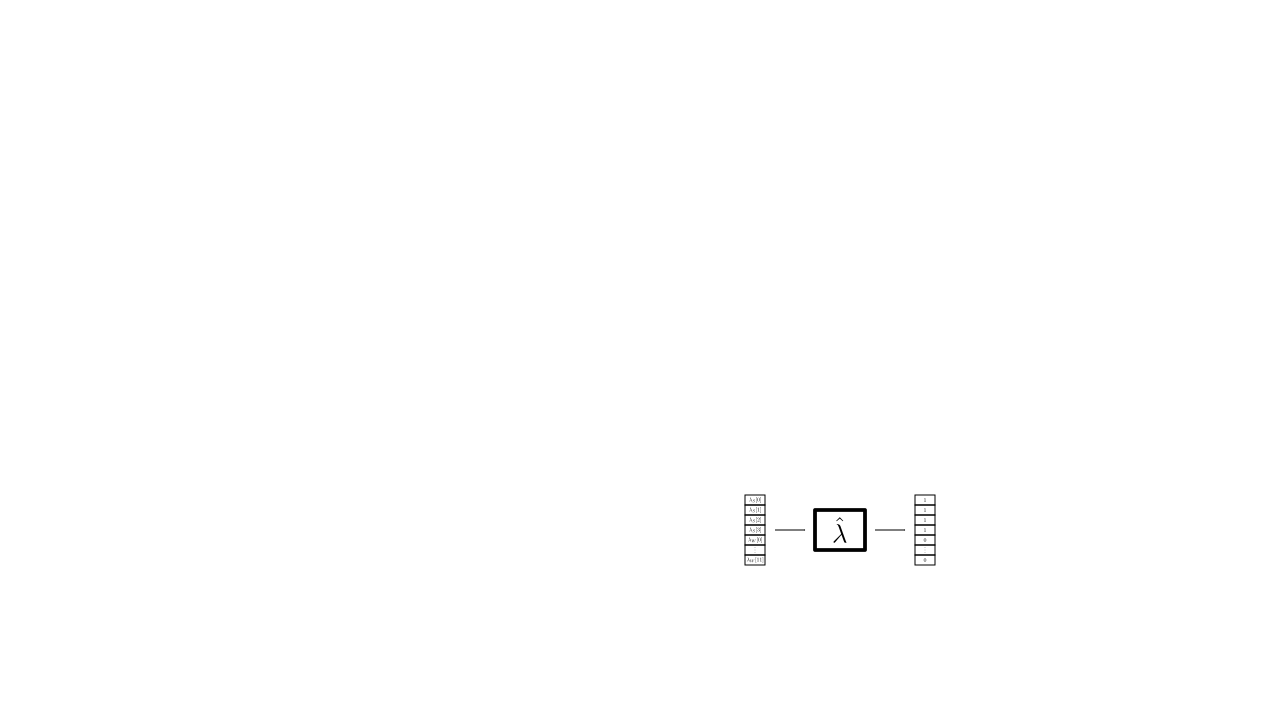
\includegraphics[width=0.7\linewidth]{images/05-Machine Learning/ml_maxder_imp.png}
  \caption{Esquema del estimador de cantidad de señales recibidas mediante el método de la máxima derivada visto como sistema para el caso de recepción de 4 señales. Se indican con $\lambda_S$ aquellos valores singulares correspondientes al subespacio de señal y con $\lambda_W$ aquellos que corresponden al subespacio de ruido.}
  \label{fig:ml_maxder_imp}
\end{figure}

Con esta simulación se compararon los vectores entregados por el algoritmo con los datos conocidos de los valores singulares clasificados para obtener una cuenta de los errores en la estimación y así obtener una medición de la precisión del algoritmo, la cual fue del 86,87\%.
%El error más probable que puede ocurrir en este algoritmo es que se detecten menos señales que las que existen en realidad. Siendo que la cantidad mínima de señales recibidas que entrega este algoritmo es 1 (ya que con alta probabilidad existirá un máximo en la derivada de la distribución), el error en esta técnica aumentará a medida que aumente la cantidad de señales recibidas. Una forma intuitiva de ver esto es pensar el caso en el que solo se recibe una única señal, en este caso el número mínimo que entregará el algoritmo será uno y esa señal será detectada el 100\% de las veces. Cuando se reciban dos señales, en el caso pesimista en el que solo se detecte una sola de ellas la precisión será del 50\%, y así sucesivamente.

\section{Clasificador binario mediante aprendizaje automático}

El problema de determinar si un valor singular corresponde al subespacio de ruido o al subespacio de señal se enmarca dentro de lo que en el campo del \emph{aprendizaje automático} o \emph{machine learning} se conoce como ``problema de clasificación binaria''.

En este tipo de problemas se intenta predecir el valor de una variable ``$y$'', de la cual se sabe que puede tomar dos valores, 0 y 1, que en este caso específico corresponden a la característica de si cada valor singular es un valor singular de ruido o de señal respectivamente, es decir:
\begin{equation}
  y=\left\{\begin{matrix}
    0 & \textrm{si corresponde a }\mathcal{S}_W \\
    1 & \textrm{si corresponde a }\mathcal{S}_S
  \end{matrix}\right.
\end{equation}
Esta predicción debe realizarse a partir de una entrada $\bar{x}$, la cual para esta aplicación en particular va a estar conformada por los parámetros que caracterizan a cada valor singular que se desea clasificar, y una hipótesis $h_{\bar{\theta}}(\bar{x})$ la cual no es más que una función que al recibir una entrada $\bar{x}$ entrega a la salida una predicción de la probabilidad de que $y$ sea igual a 1 para dicha entrada y para una elección de coeficientes representados en los elementos de un vector $\bar{\theta}$. Luego, configurando el umbral correspondiente, puede considerarse como $y=1$ a valores de probabilidad por encima de 0,5 y viceversa, y de esta forma se tiene el sistema clasificador que se indica en la Figura \ref{fig:ml_classificator_system}.
\begin{figure}[ht!]
  \centering
  
\includegraphics[width=0.7\linewidth]{images/05-Machine Learning/ml_classificator_system.png}
  \caption{Esquema de un clasificador utilizando aprendizaje automático visto como sistema.}
  \label{fig:ml_classificator_system}
\end{figure}

Existen varios tipos de algoritmos clasificadores, los cuales cada uno define su propia función de hipótesis $h_{\bar{\theta}}(\bar{x})$. A lo largo de este capítulo se analizarán dos de estos tipos; en primer lugar se explicará la técnica de \emph{Regresión Logística} para dar una introducción a los conceptos relacionados con el aprendizaje automático, y, finalmente, se analizará el algoritmo conocido como \emph{Máquina de Vectores de Soporte}, el cual es el algoritmo que finalmente se escogió para la implementación de este proyecto.

\subsection{Regresión Logística}
Debido a que la salida del clasificador es una variable que se encuentra contenida dentro del rango $[0,1]$ hay que definir una función para $h_{\bar{\theta}}(\bar{x})$ que cumpla con esta característica. El algoritmo de Regresión Logística define la siguiente función de hipótesis \cite{bib:machinelearning}:
\begin{gather}
  h_{\bar{\theta}}(\bar{x})=g(\bar{\theta}^T \bar{x}),\\
  g(z)=\frac{1}{1+e^{-z}},\end{gather}
donde $g(z)$ es conocida como la \emph{función sigmoide} o \emph{función lógística}, cuya forma se muestra en la Figura \ref{fig:ml_sigmoid}, y $\bar{\theta}$ es un vector de coeficientes a determinar.
\begin{figure}[ht!]
  \centering
  \includegraphics[width=0.9\linewidth]{images/05-Machine Learning/ml_sigmoid.png}
  \caption{Gráfica de la función sigmoide.}
  \label{fig:ml_sigmoid}
\end{figure}
Como se ve, esta función tiende a 1 para $z\rightarrow \infty$ y a 0 para $z\rightarrow -\infty$, y para $z=0$ vale 0,5.

El objetivo de todos los algoritmos de aprendizaje automático es el de ajustar los elementos del vector $\bar{\theta}$ de manera tal que la hipótesis genere una frontera de decisión que permita clasificar con la mayor precisión posible un conjunto de datos representados como vectores $\bar{x}$. Por ejemplo, si tenemos el conjunto de datos que se muestra en la Figura \ref{fig:ml_dataexample} se pueden definir los vectores:
\begin{equation*}
  \bar{x}=\begin{bmatrix}
    1     \\
    x_1   \\
    x_2   \\
    x_1^2 \\
    x_2^2
  \end{bmatrix},\quad
  \bar{\theta}=\begin{bmatrix}
    -1 \\
    0  \\
    0  \\
    1  \\
    1
  \end{bmatrix},
\end{equation*}
y de esta manera manera se tiene una función de hipótesis definida por:
\begin{equation*}
  h_{\bar{\theta}}(\bar{x})=g(\theta_0+\theta_1 x_1 + \theta_2 x_2 + \theta_3 x_1^2 + \theta_4 x_2^2) = g(-1+x_1^2+x_2^2)
\end{equation*}

Debido a lo que se ve en la Figura \ref{fig:ml_sigmoid}, la función sigmoide devuelve valores por encima de 0,5 para entradas mayores a 0. Por esto, para encontrar la frontera de decisión basta con ver los puntos del argumento de $g(\bar{\theta}^T \bar{x})$ tal que:
\begin{equation*}
  \bar{\theta}^T \bar{x} = -1+x_1^2+x_2^2 = 0,
\end{equation*}
y esos puntos son los que definen la frontera circular que se muestra en la Figura \ref{fig:ml_dataexample}.
\begin{figure}[ht!]
  \centering
  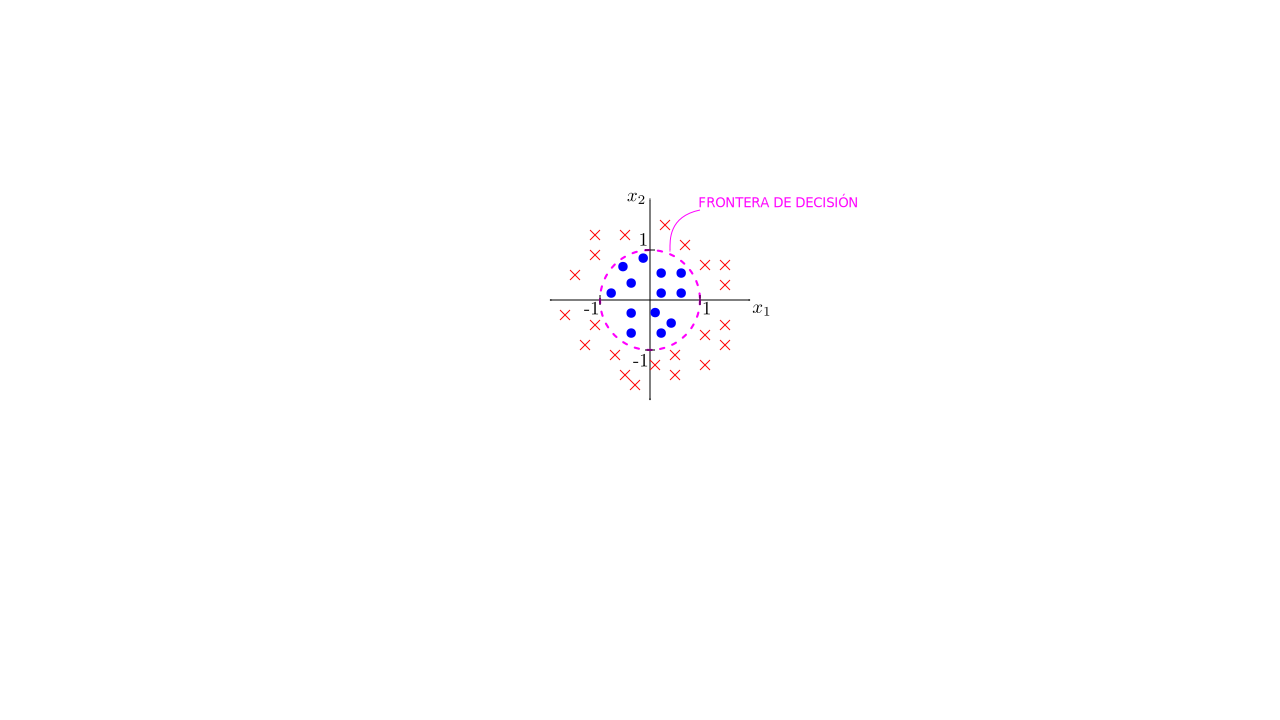
\includegraphics[width=0.8\linewidth]{images/05-Machine Learning/ml_dataexample.png}
  \caption{Ejemplo de frontera de decisión para un problema de clasificación binaria.}
  \label{fig:ml_dataexample}
\end{figure}

Vale la pena notar que en el ejemplo de la Figura \ref{fig:ml_dataexample} los datos a clasificar dependen de dos parámetros: $x_1$ y $x_2$. Sin embargo, el vector $\bar{x}$ no contiene únicamente estos dos parámetros sino que agrega nuevas \emph{características}, como lo son un término independiente $x_0=1$ y dos parámetros más que dependen de los originales: $x_1^2$ y $x_2^2$. Este método de agregar características polinomiales o términos rectangulares permite lograr fronteras de decisión más complejas que ajusten mejor a un determinado conjunto de datos, aunque pueden provocar un ``sobreajuste'' de los parámetros que degrade el comportamiento del clasificador al trabajar con datos que se encuentren fuera del conjunto de entrenamiento.

Como se dijo, el objetivo del aprendizaje automático consiste en ajustar los valores de $\bar{\theta}$ de manera tal de encontrar una frontera de decisión óptima. La manera de realizar este ajuste es entrenando al algoritmo a partir de un conjunto de datos llamado \emph{conjunto de entrenamiento}, de manera tal que, a medida de que el algoritmo itere, el error en la clasificación se reduzca. Para esto hay que definir una métrica de ese error, la cual es conocida como \emph{función de costo}. Para el algoritmo de regresión logística y teniendo un conjunto de datos de tamaño $M$ y una cantidad de características $N$, la función de costo está definida por \cite{bib:machinelearning}:
\begin{equation}
  J(\bar{\theta},\lambda)= -\frac{1}{M}\sum_{i=0}^{M-1} \left[y^{(i)} \log\left(h_{\bar{\theta}}(\bar{x}^{(i)})\right) + (1-y^{(i)}) \log\left(1-h_{\bar{\theta}}(\bar{x}^{(i)})\right) \right]+\frac{\lambda}{2M}\sum_{j=1}^{N-1}\theta_j^2,
  \label{eq:ml_costfunction}
\end{equation}
donde $y^{(i)}$ es la $i$-ésima variable que se desea predecir, $\bar{x}^{(i)}$ es el vector de entrada del clasificador correspondiente a la $i$-ésima variable a predecir, $\lambda$ es el \emph{parámetro de regularización} que permite suavizar la salida de la función de hipótesis para reducir el sobreajuste. Este parámetro también debe ser ajustado mediante entrenamiento. Finalmente, el problema a resolver consiste en encontrar los valores de $\bar{\theta}$ y $\lambda$ que minimicen la función de costo, es decir:
\begin{equation}
  \min_{\bar{\theta},\lambda} J(\bar{\theta},\lambda)
\end{equation}

Para minimizar la función de costo en regresión logística el procedimiento que se utiliza es el método de \emph{descenso de gradiente}, el cual es un algoritmo iterativo que permite acercarse con una cierta velocidad al mínimo de una función derivable. Utilizando esta técnica, la actualización de parámetros por cada iteración viene dada por:
\begin{equation}
  \begin{split}
    \theta_0 &:= \theta_0- \frac{\alpha}{M} \sum_{i=0}^{M-1}\left(h_{\bar{\theta}}(\bar{x}^{(i)})-y^{(i)}\right)x_0^{(i)}\\
    \theta_j &:= \theta_j- \frac{\alpha}{M} \left[\sum_{i=0}^{M-1} \left(h_{\bar{\theta}}(\bar{x}^{(i)})-y^{(i)}\right)x_j^{(i)}+\lambda\theta_j \right]\quad \textrm{para } j=1,...,N-1,
  \end{split}
\end{equation}
donde $\alpha$ es el \emph{coeficiente de aprendizaje} el cual se encarga de definir el tamaño de los ``pasos'' que se dan cuesta abajo en cada iteración del algoritmo. Si este $\alpha$ se elige muy grande es posible que el algoritmo nunca converja, y si se elige muy pequeño puede que tarde mucho tiempo en converger.
Es necesario ver que con este método no se actualiza el valor del parámetro $\lambda$. La manera de elegir un valor óptimo para este parámetro consiste en entrenar el algoritmo utilizando distintos valores de $\lambda$ y luego observar el rendimiento del clasificador utilizando datos que se encuentran fuera del conjunto de entrenamiento, eligiendo, finalmente, el valor de $\lambda$ que mejor ajuste este nuevo conjunto de datos, el cual es llamado \emph{conjunto de validación}.

\subsection{Máquina de Vectores de Soporte}\label{subc:ml_svm}
Uno de los algoritmos de clasificación más utilizados tanto en la industria como en la academia es el conocido como \emph{Máquina de Vectores de Soporte} (o \emph{SVM}, por sus siglas en inglés), el cual tiene la capacidad de poder entregar una mejor elección de una frontera de decisión a un menor costo comparado con el algoritmo de Regresión Logística. El algoritmo SVM toma la función de costos de la Ecuación \ref{eq:ml_costfunction}, y la simplifica de la siguiente manera:
\begin{equation}
  J(\bar{\theta},C)= C\sum_{i=0}^{M-1} \left[y^{(i)} \mathrm{cost}_1 (\bar{\theta}^T \bar{x}^{(i)}) + (1-y^{(i)}) \mathrm{cost}_0 (\bar{\theta}^T \bar{x}^{(i)}) \right]+\frac{1}{2}\sum_{j=1}^{N-1}\theta_j^2
  \label{eq:ml_costfunction_svm}
\end{equation}
donde $\mathrm{cost}_0(z)$ y $\mathrm{cost}_1(z)$ son las funciones que se indican en la Figura \ref{fig:ml_cost_svm} y $C = \frac{1}{\lambda}$.
\begin{figure}[ht!]
  \centering
  \begin{subfigure}[b]{0.49\textwidth}
    \centering
    \includegraphics[width=\linewidth]{images/05-Machine Learning/ml_cost1.png}
    \caption{$\mathrm{cost}_1(z)$}
  \end{subfigure}
  \hfill
  \begin{subfigure}[b]{0.49\textwidth}
    \centering
    \includegraphics[width=\linewidth]{images/05-Machine Learning/ml_cost0.png}
    \caption{$\mathrm{cost}_0(z)$}
  \end{subfigure}
  \caption{Cambios en la función de costo para SVM.}
  \label{fig:ml_cost_svm}
\end{figure}

Otra diferencia que tiene SVM con respecto a Regresión Logística es que la función de hipótesis en este caso no entrega una probabilidad sino directamente la predicción de $y$, es decir:
\begin{equation}
  h_{\bar{\theta}}(\bar{x})=\left\{\begin{matrix}
    0 & \textrm{si }\bar{\theta}^T \bar{x} < 0    \\
    1 & \textrm{si }\bar{\theta}^T \bar{x} \geq 0
  \end{matrix}\right.
  \label{eq:ml_hip_svm}
\end{equation}

Si se analizan la funciones $\mathrm{cost}_0(z)$ y $\mathrm{cost}_1(z)$ que se muestran en la Figura \ref{fig:ml_cost_svm} puede verse que la condición para que el primer término de la función de costos definida en la Ecuación \ref{eq:ml_costfunction_svm} se anule es:
\begin{equation}
  \begin{matrix}
    \bar{\theta}^T \bar{x}^{(i)}  \geq & 1  & \textrm{si } y^{(i)} = 1, \\
    \bar{\theta}^T \bar{x}^{(i)}  \leq & -1 & \textrm{si } y^{(i)} = 0.
  \end{matrix}
  \label{eq:ml_cond_svm}
\end{equation}

Cuando se resuelve el problema de optimización de minimizar la Ecuación \ref{eq:ml_costfunction_svm} resulta que la frontera de decisión que se obtiene utilizando SVM maximiza la distancia entre ella y los datos más cercanos a ella de cada una de las dos clases. Para dar un ejemplo de esto se muestra el conjunto de entrenamiento de la Figura \ref{fig:ml_db_svm}. Aquí vemos que en este caso de clasificación lineal pueden generarse infinitas rectas que logren una perfecta clasificación de este conjunto de datos, como las indicadas por las fronteras de color verde, sin embargo la frontera definida por SVM induce a pensar que va a lograr un mejor trabajo clasificando datos nuevos.
\begin{figure}[ht!]
  \centering
  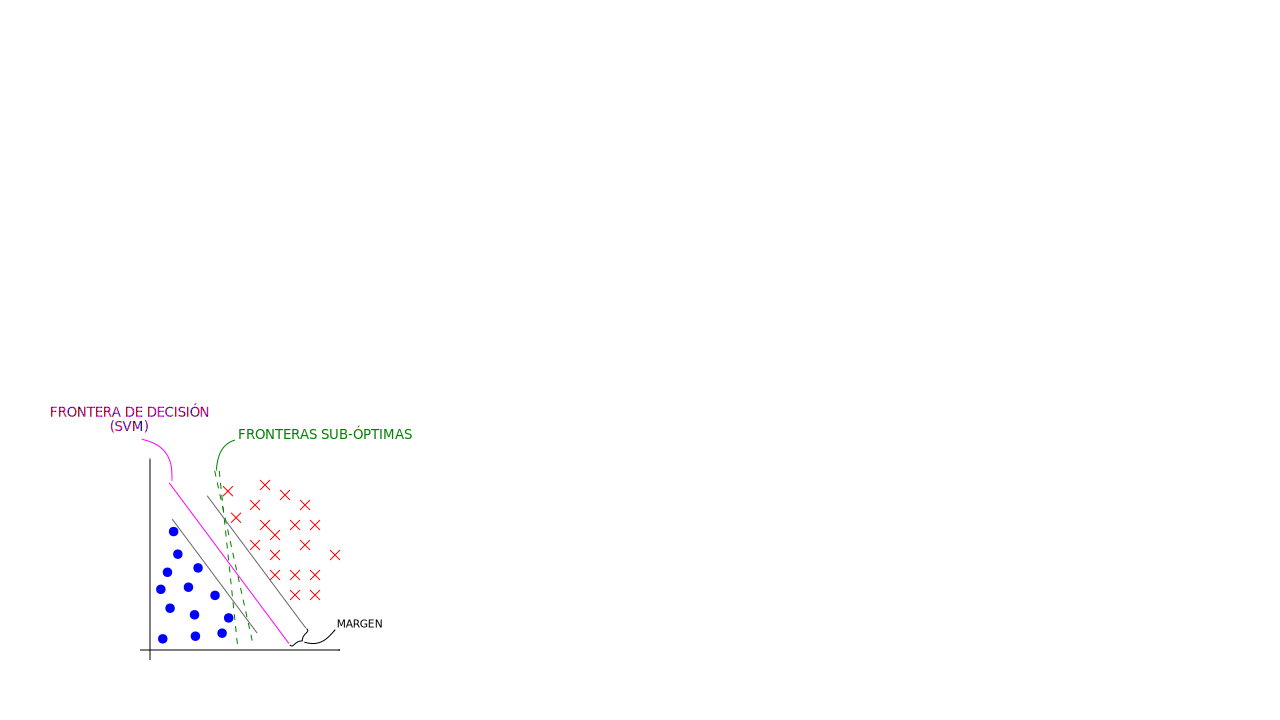
\includegraphics[width=0.8\linewidth]{images/05-Machine Learning/ml_db_svm.png}
  \caption{Frontera de decisión utilizando SVM.}
  \label{fig:ml_db_svm}
\end{figure}

De la Figura \ref{fig:ml_db_svm} se observa también que la frontera de decisión generada por SVM es la que maximiza el margen de separación entre datos rojos y azules. La razón por la cual ocurre esto tiene que ver con la condición definida en la Ecuación \ref{eq:ml_cond_svm} y la función de costos de la Ecuación \ref{eq:ml_costfunction_svm} ya que cumpliendo esas condiciones tenemos que la función de costo queda definida por:
\begin{equation}
  J(\bar{\theta})=\frac{1}{2} \sum_{j=1}^{N-1}\theta_j^2=\frac{1}{2} \left \|\bar{\theta} \right \|^2.
  \label{eq:ml_j_cost0}
\end{equation}
Además, las condiciones de la Ecuación \ref{eq:ml_cond_svm} pueden reescribirse como:
\begin{equation}
  \begin{matrix}
    p^{(i)} \cdot \left \| \bar{\theta} \right \| \geq & 1  & \textrm{si } y^{(i)} = 1, \\
    p^{(i)} \cdot \left \| \bar{\theta} \right \|\leq  & -1 & \textrm{si } y^{(i)} = 0,
  \end{matrix}
  \label{eq:ml_proyeccion_svm}
\end{equation}
donde $p^{(i)}$ es la proyección del vector $\bar{x}^{(i)}$ sobre el vector $\bar{\theta}$, o, lo que es lo mismo, la distancia del dato $\bar{x}^{(i)}$ a la frontera de decisión, debido a que la frontera de decisión es perpendicular a $\bar{\theta}$. Esto puede verse en el ejemplo de la Figura \ref{fig:ml_proyeccion_svm}.
\begin{figure}[ht!]
  \centering
  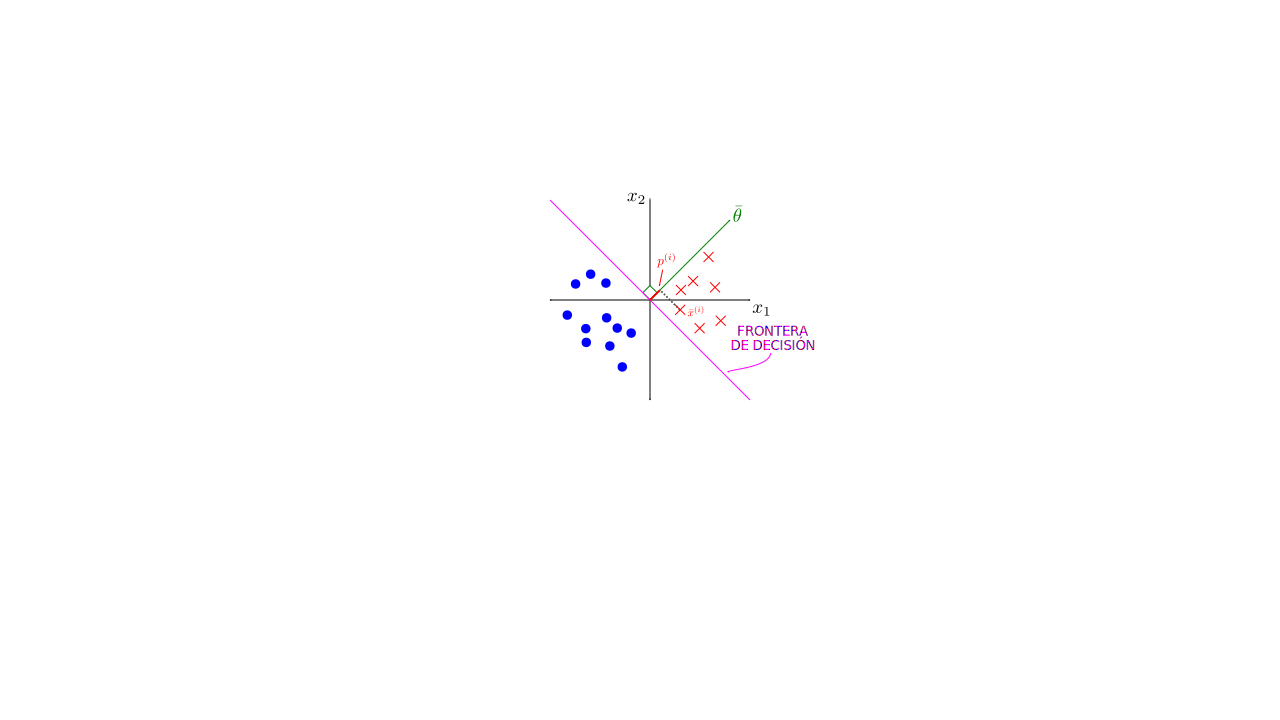
\includegraphics[width=0.7\linewidth]{images/05-Machine Learning/ml_proyeccion_svm.png}
  \caption{Proyección de un dato $\bar{x}^{(i)}$ sobre el vector $\bar{\theta}$ para un clasificador lineal con $\theta_0=0$.}
  \label{fig:ml_proyeccion_svm}
\end{figure}
Si algún dato $\bar{x}^{(i)}$ se encontrara sobre la frontera de decisión estaría ubicado numéricamente en el salto de la función de hipótesis definida en la Ecuación \ref{eq:ml_hip_svm}, lo que significa que para puntos definidos por vectores $\bar{x}^{(i)}$ que se encuentren dentro de la frontera de decisión, el producto escalar $\bar{\theta}^T \bar{x}$ vale 0, lo que indica que todos los puntos dentro de la frontera de decisión son ortogonales a $\bar{\theta}$.

A partir de aquí se observa que al minimizar la Ecuación \ref{eq:ml_j_cost0} se minimiza la norma de $\bar{\theta}$, por ende para cumplir las condiciones de la Ecuación \ref{eq:ml_proyeccion_svm} al minimizarse $\left\| \bar{\theta} \right \|$ debe maximizarse $p^{(i)}$, lo que significa maximizar la distancia entre los datos del conjunto de entrenamiento y la frontera de decisión.

Finalmente, SVM implementa una nueva manera de definir las características del vector $\bar{x}$ distinta a la manera polinomial que se vio en Regresión Logística. Teniendo un conjunto de $M$ datos de entrenamiento se define el vector de características de un dato $\bar{f}^{(i)}\in \mathbb{R}^{M\times 1}$ para $i=0,1,...,M-1$ como:
\begin{equation}
  \bar{f}^{(i)}=\begin{bmatrix}
    f_0^{(i)} \\
    f_1^{(i)} \\
    \vdots    \\
    f_{M-1}^{(i)}
  \end{bmatrix}_{(M\times 1)} ,
\end{equation}
donde $f_j^{(i)}=k(\bar{x}^{(i)},\bar{x}^{(j)})$ es una función que mide la ``semejanza'' entre el dato $\bar{x}^{(i)}$ y el dato $\bar{x}^{(j)}$, la cual es llamada \emph{función kernel}. Ahora la función de hipótesis queda definida por:
\begin{equation}
  h_{\bar{\theta}}(\bar{f})=\left\{\begin{matrix}
    0 & \textrm{si }\bar{\theta}^T \bar{f} < 0    \\
    1 & \textrm{si }\bar{\theta}^T \bar{f} \geq 0
  \end{matrix}\right.
  \label{eq:ml_hipkernel_svm}
\end{equation}

Debe notarse que ahora la dimensión del vector $\bar{\theta}$ es igual a la cantidad de datos del conjunto de entrenamiento, entonces la función de costo de la Ecuación \ref{eq:ml_costfunction} puede reescribirse como:
\begin{equation}
  J(\bar{\theta},C)= C\sum_{i=0}^{M-1} \left[y^{(i)} \mathrm{cost}_1 (\bar{\theta}^T \bar{f}^{(i)}) + (1-y^{(i)}) \mathrm{cost}_0 (\bar{\theta}^T \bar{f}^{(i)}) \right]+\frac{1}{2}\sum_{j=1}^{M-1}\theta_j^2
  \label{eq:ml_costfunctionkernel_svm}
\end{equation}

Existen múltiples maneras de definir la función kernel, donde cada una se ajusta mejor a ciertos tipos de distribuciones de datos. Algunos de los tipos de kernels más comunes son \cite{bib:sklearn_svm}:
\begin{itemize}
  \item \textbf{Kernel Lineal :=} $k_{\textrm{lineal}}(\bar{x}^{(i)},\bar{x}^{(j)})=\left \langle \bar{x}^{(i)},\bar{x}^{(j)} \right \rangle$
  \item \textbf{Kernel Gaussiano :=} $k_{\textrm{gaussiano}}(\bar{x}^{(i)},\bar{x}^{(j)})=-\gamma \left \| \bar{x}^{(i)}-\bar{x}^{(j)} \right \|^2$, con $\gamma>0$
  \item \textbf{Kernel Polinomial :=} $k_{\textrm{polinomial}}(\bar{x}^{(i)},\bar{x}^{(j)})=\left( \gamma \left \langle \bar{x}^{(i)},\bar{x}^{(j)} \right \rangle +r \right)^d$, siendo $d$ el grado del polinomio y $r$ un término independiente.
  \item \textbf{Kernel Sigmoide :=} $k_{\textrm{sigmoide}}(\bar{x}^{(i)},\bar{x}^{(j)})=\tanh{\left(\gamma \left \langle \bar{x}^{(i)},\bar{x}^{(j)} \right \rangle +r\right)}$

\end{itemize}

En la actualidad existen múltiples librerías con implementaciones optimizadas de algoritmos de SVM para distintos tipos de kernels escritos en una gran variedad de lenguajes, como lo son la librería \texttt{scikit-learn} \cite{bib:sklearn_svm} en \texttt{Python} o \texttt{LIBSVM} \cite{bib:LIBSVM} en \texttt{C++}, lo cual hace que la implementación de estos algoritmos pueda realizarse de forma muy rápida.

\subsection{Resultados obtenidos}
%Feature scaling
% Método de testeo: training set - cross validations set - test set
% 6 week
%Training set: 60%
%Cross validation set: 20%
%Test set: 20% 

En esta sección se muestran los resultados obtenidos luego de aplicar las técnicas de estimación de cantidad de señales recibidas mediante aprendizaje automático. En este caso solo se realizó el análisis del algoritmo SVM debido a su simplicidad de implementación con respecto a Regresión Logística.

Para poder operar con estas técnicas primero deben elegirse las características que definen a cada valor singular a clasificar. La primer característica a definir es la magnitud del mismo, ya que cuanto más grande sea, mayor va a ser la probabilidad de que sea un valor singular correspondiente al subespacio de señal. Sin embargo esta característica no es suficiente, ya que, según cómo sean las propiedades de las señales recibidas, el piso de ruido puede variar de manera tal de que lo que antes era una magnitud que correspondía a un valor singular de señal en otro caso puede corresponder a un valor singular de ruido. Por ende hay que definir una nueva característica que tenga en cuenta la relación de magnitudes entre los valores singulares de ruido y de señal en cada descomposición de valores singulares. Según lo que se definió en la Ecuación \ref{eq:doaest_aval}, en la descomposición en autovalores de la matriz $\mathbf{R_{XX}}$ definida en la Ecuación \ref{eq:doaest_rxx_teor} los autovalores máximos y mínimos vienen dados por:
\begin{align}
  \lambda_{\textrm{máx}} & = M \cdot |s_{\textrm{máx}}|^2+\sigma_w^2, \\
  \lambda_{\textrm{mín}} & = \sigma_w^2.
\end{align}
Por ende, a partir de estos valores puede definirse una noción de SNR haciendo:
\begin{equation}
  \hat{\mathrm{SNR}} = \frac{\lambda_{\textrm{máx}}-\lambda_{\textrm{mín}}}{M\cdot \lambda_{\textrm{mín}}}=\frac{|s_{\textrm{máx}}|^2}{\sigma_w^2}
  \label{eq:ml_svm_snrhat}
\end{equation}
Hay que tener en cuenta que esta definición no indica una SNR per se, ya que $\lambda_{\textrm{máx}}$ solo contiene información de la señal que arriba con mayor potencia e ignora a las otras, pero esta diferencia de magnitudes permite aportar información de utilidad que permita realizar la clasificación de los valores singulares. Además, siendo que se trabaja con una cantidad de muestras finitas, los autovalores de la matriz de covarianza muestral definida en la Ecuación \ref{eq:doaest_rxx_est} no serán iguales a lo que se mostró en la Ecuación \ref{eq:doaest_aval} y ocurrirá que los autovalores de ruido contendrán información de las señales y viceversa. Sin embargo, la práctica demuestra que es una buena métrica que puede usarse como característica. Como en la Sección \ref{subc:doaest_datamodel} se decidió que la descomposición del subespacio se realiza aplicando directamente la SVD sobre la matriz $\mathbf{X}$ definida en la Ecuación \ref{eq:doaest_x}, no se puede definir exactamente la misma SNR de la Ecuación \ref{eq:ml_svm_snrhat}, ya que los valores singulares de $\mathbf{X}$ no son iguales a los autovalores de $\mathbf{\hat{R}_{XX}}$, sin embargo, estos están relacionados de la siguiente manera \cite{bib:strang}:
\begin{equation}
  \sigma_{\mathbf{X}} = \sqrt{|\lambda_{\mathbf{\hat{R}_{XX}}}|},
\end{equation}
siendo $\sigma_{\mathbf{X}}$ los valores singulares de $\mathbf{X}$ y $\lambda_{\mathbf{\hat{R}_{XX}}}$ los autovalores de $\mathbf{\hat{R}_{XX}}$. Entonces, utilizando los valores singulares de la SVD de $\mathbf{X}$ se puede redefinir la SNR de la Ecuación \ref{eq:ml_svm_snrhat} de la siguiente forma:
\begin{equation}
  \hat{\mathrm{SNR}} = \frac{\sigma^2_{\textrm{máx}}}{\sigma^2_{\textrm{mín}}},
  \label{eq:ml_svm_snrhatsvd}
\end{equation}
donde $\sigma_{\textrm{máx}}$ y $\sigma_{\textrm{mín}}$ son los valores singulares máximos y mínimos, respectivamente, de cada SVD realizada sobre cada matriz de muestras $\mathbf{X}$.

A partir de estas dos características ahora puede definirse un vector de entrada para el clasificador de la siguiente manera:
\begin{equation}
  \bar{x}^{(i)}=\begin{bmatrix}
    \lambda^{(i)} \\
    \hat{\mathrm{SNR}}^{(i)}
  \end{bmatrix}
  \label{eq:ml_svm_x}
\end{equation}
con $i=0,1,...,M-1$, y siendo $M$ el tamaño del conjunto de datos.

Utilizando la misma base de valores singulares que se generó en la Sección \ref{subc:ml_maxder_resul} y en función de la definición de la Ecuación \ref{eq:ml_svm_x}, puede realizarse la gráfica de la Figura \ref{fig:ml_avals_plot}, en donde se representan 2000 valores singulares correspondientes al subespacio de ruido y 2000 valores singulares correspondientes al subespacio de señal elegidos al azar en función de las características definidas. Como puede verse en esta gráfica, existen dos zonas bien separadas que pueden utilizarse para definir una frontera de decisión. Los valores singulares de ruido se ubican sobre el margen izquierdo de la gráfica, la cual corresponde a valores singulares de magnitud pequeña, y los autovalores de señal se extienden por toda la gráfica hacia la derecha, tomando diferentes valores según la potencia de la señal que representan.
\begin{figure}[ht!]
  \centering
  \includegraphics[width=0.9\linewidth]{images/05-Machine Learning/ml_avals_plot.png}
  \caption{Gráfica de valores singulares de distintas realizaciones de $\mathbf{X}$ en función de las características definidas para el problema de clasificación mediante aprendizaje automático.}
  \label{fig:ml_avals_plot}
\end{figure}

Antes de comenzar con el entrenamiento del algoritmo es necesario preparar los datos para que las iteraciones minimicen la función de costo de la manera más rápida. Para lograr esto se utilizará la técnica de \emph{escalamiento de características} \cite{bib:machinelearning}, que consiste en normalizar los rangos de variación de los valores de las características del conjunto de entrenamiento para que ambos varíen en una misma escala. Para eso se procede definiendo las siguientes magnitudes:
\begin{equation}
  \begin{gathered}
    \mu_{\lambda}=\frac{1}{M_{\textrm{tr}}} \sum_{i=0}^{M_{\textrm{tr}-1}} \lambda^{(i)},\quad \mu_{\hat{\mathrm{SNR}}}=\frac{1}{M_{\textrm{tr}}} \sum_{i=0}^{M_{\textrm{tr}-1}} \hat{\mathrm{SNR}}^{(i)}\\
    \sigma_{\lambda}=\max(\bar{\lambda})-\min(\bar{\lambda}),\quad \sigma_{\hat{\mathrm{SNR}}}=\max(\bar{\mathrm{SNR}})-\min(\bar{\mathrm{SNR}}),
  \end{gathered}
\end{equation}
donde $\mu_{\lambda}$ es el valor medio de las magnitudes de todos los valores singulares en el conjunto de entrenamiento, $\mu_{\hat{\mathrm{SNR}}}$ es el valor medio de la $\hat{\mathrm{SNR}}$ de todos los valores singulares del conjunto de entrenamiento como se definió en la Ecuación \ref{eq:ml_svm_snrhat}, $\sigma_{\lambda}$ es la diferencia entre la magnitud del valor singular máximo y mínimo del conjunto de entrenamiento, $\sigma_{\hat{\mathrm{SNR}}}$ es la diferencia entre el valor de $\hat{\mathrm{SNR}}$ máximo y mínimo de todo el conjunto de entrenamiento, y $M_{\textrm{tr}}$ es el tamaño del conjunto de entrenamiento. Luego de definir estas variables se afecta a cada vector $\bar{x}^{(i)}$ del conjunto total de datos de la siguiente manera:
\begin{gather}
  \bar{x}_{fs}^{(i)}=\mathbf{\Sigma} \cdot \left( \bar{x}^{(i)} - \bar{\mu}  \right)=\begin{bmatrix}
    \frac{\lambda^{(i)}-\mu_{\lambda}}{\sigma_{\lambda}} \\
    \frac{\hat{\mathrm{SNR}}-\mu_{\hat{\mathrm{SNR}}}}{\sigma_{\hat{\mathrm{SNR}}}}
  \end{bmatrix}\\
  \mathbf{\Sigma}=\begin{bmatrix}
    \frac{1}{\sigma_{\lambda}} & 0                                     \\
    0                          & \frac{1}{\sigma_{\hat{\mathrm{SNR}}}}
  \end{bmatrix},\quad \bar{\mu}=\begin{bmatrix}
    \mu_{\lambda} \\
    \mu_{\hat{\mathrm{SNR}}}
  \end{bmatrix}\nonumber
\end{gather}


Luego de acondicionar los datos se definieron los conjuntos de entrenamiento, validación y prueba de la siguiente manera:
\begin{itemize}
  \item \textbf{Conjunto de entrenamiento:} 60\% del conjunto total de datos. Es el utilizado para obtener los elementos del vector de parámetros $\bar{\theta}$ mediante entrenamiento del algoritmo.
  \item \textbf{Conjunto de validación:} 20\% del conjunto total de datos. Se utiliza para ajustar los coeficientes y términos independientes propios de cada kernel.
  \item \textbf{Conjunto de prueba}: 20\% del conjunto total de datos. Se utiliza para medir la precisión del algoritmo.
\end{itemize}

Utilizando los conjuntos de entrenamiento y validación se entrenó el algoritmo SVM utilizando distintos kernels, obteniendo los resultados que se muestran a continuación.

\subsubsection{Kernel Sigmoide}

Luego de entrenar al algoritmo utilizando este kernel se llegó a la elección de parámetros $C=30$, $\gamma=0,3$ y $r=0,01$. A partir de estos parámetros y la obtención del vector $\bar{\theta}$ mediante entrenamiento del algoritmo se obtuvo la frontera de decisión que se muestra en la Figura \ref{fig:ml_svm_sigmoid}.

\begin{figure}[ht!]
  \centering
  \includegraphics[width=0.9\linewidth]{images/05-Machine Learning/ml_svm_sigmoid.png}
  \caption{Frontera de decisión definida por el algoritmo SVM utilizando un kernel sigmoide}
  \label{fig:ml_svm_sigmoid}
\end{figure}

Comparando las características conocidas del conjunto de datos se evaluó la precisión del clasificador utilizándolo en distintos conjuntos de prueba obteniendo los siguientes resultados:
\begin{itemize}
  \item \textbf{Conjunto de prueba:} 96,70\% de precisión.
  \item \textbf{Conjunto de validación:} 96,60\% de precisión.
  \item \textbf{Conjunto de entrenamiento:} 96,71\% de precisión.
  \item \textbf{Todos los datos:} 96,69\% de precisión.
\end{itemize}

\subsubsection{Kernel Polinomial}
Realizando numerosas iteraciones se optimizó el algoritmo SVM utilizando un kernel polinomial con los parámetros $C=0,03$, $d=4$, $\gamma=50$, $r=1$. En la Figura \ref{fig:ml_svm_poly} se muestra la frontera de decisión obtenida con este clasificador. Como puede observarse, esta frontera no pareciera mostrar un resultado adecuado en la zona inferior izquierda e inferior derecha de la gráfica, esto se debe a la falta de valores singulares en esa zona que ayuden a aportar información al algoritmo.

\begin{figure}[ht!]
  \centering
  \includegraphics[width=0.9\linewidth]{images/05-Machine Learning/ml_svm_poly.png}
  \caption{Frontera de decisión definida por el algoritmo SVM utilizando un kernel polinomial.}
  \label{fig:ml_svm_poly}
\end{figure}

\begin{itemize}
  \item \textbf{Conjunto de prueba:} 96,85\% de precisión.
  \item \textbf{Conjunto de validación:} 97,15\% de precisión.
  \item \textbf{Conjunto de entrenamiento:} 96,92\% de precisión.
  \item \textbf{Todos los datos:} 96,95\% de precisión.
\end{itemize}

\subsubsection{Kernel Gaussiano}
Luego de entrenar al algoritmo se fijaron los parámetros $C=50$ y $\gamma=30$. En la Figura \ref{fig:ml_svm_rbf} se indica la frontera de decisión definida por este kernel junto con el conjunto de datos clasificado.

\begin{figure}[ht!]
  \centering
  \includegraphics[width=0.9\linewidth]{images/05-Machine Learning/ml_svm_rbf.png}
  \caption{Frontera de decisión definida por el algoritmo SVM utilizando un kernel gaussiano.}
  \label{fig:ml_svm_rbf}
\end{figure}

Contando los errores producidos al clasificar los distintos conjuntos de datos se obtuvieron las siguientes medidas de precisión:
\begin{itemize}
  \item \textbf{Conjunto de prueba:} 96,92\% de precisión.
  \item \textbf{Conjunto de validación:} 97,25\% de precisión.
  \item \textbf{Conjunto de entrenamiento:} 97,12\% de precisión.
  \item \textbf{Todos los datos:} 97,11\% de precisión.
\end{itemize}

Con las simulaciones realizadas puede concluirse que este es el kernel que alcanzó la mayor precisión. Sin embargo, el entrenamiento del algoritmo con datos simulados no es suficiente para llevar este clasificador a una implementación real. En ese caso lo correcto será volver a entrenar al mismo utilizando mediciones reales de las señales satelitales que se desea recibir.
\chapter{Detalles del sistema}\label{ch:sistema}
%\chapterquote{Hablaban siempre de dinero y planeaban asaltar un banco}{Domingo Cavallo, 2001}

\section{Esquema de bloques}\label{sec:sistema_bloques}

\section{Muestreador aleatorio}\label{sec:sistema_randomsampler}

\section{Estimador de dirección de arribo}\label{sec:sistema_doa_estimator}

\section{Conformador de haz}\label{sec:sistema_beamformer}




\chapter{GNURadio}\label{ch:gnuradio}
%\chapterquote{Hablaban siempre de dinero y planeaban asaltar un banco}{Domingo Cavallo, 2001}

\section{Conceptos generales}\label{subc:intro_congen}



%\chapter{Implementación en FPGA}\label{ch:fpga}
%\chapterquote{Hablaban siempre de dinero y planeaban asaltar un banco}{Domingo Cavallo, 2001}

\section{Conceptos generales}\label{subc:fpga_congen}



\chapter{Trabajo a futuro}\label{ch:futuro}
%\chapterquote{Hablaban siempre de dinero y planeaban asaltar un banco}{Domingo Cavallo, 2001}

\section{Innovación en la estimación}\label{subc:futuro_innovacion}

\section{Interfaz con el sistema de adquisición}\label{subc:futuro_interfaz}

\section{Empaquetamiento}\label{subc:futuro_packet}

\section{Medición del patrón de radiación del arreglo}\label{subc:futuro_patron}

\section{Interferencias destructivas}
Generación de pesos en los array para generar interferencias destructivas en direcciones donde arriban señales secundarias.

\section{Smart Beamforming}\label{subc_smartbeamforming}
Más allá que el algoritmo que se desarrolló en este proyecto puede considerarse de alguna manera ``inteligente'' debido a que es capaz de deducir por su cuenta la dirección de arribo de señales, el término \textbf{Smart Beamforming} refiere a técnicas de conformación de haz que utilizan algoritmos de inteligencia artificial para la estimación de dirección de arribo y la conformación de las señales arribantes.
\chapter{Conclusiones}\label{ch:conclusiones}
\chapterquote{He llegado hasta el fin, con los brazos cansados...}{Gustavo Cerati}

En este proyecto se realizó el estudio de distintas técnicas de implementación de un conformador de haz digital adaptativo, partiendo de una introducción teórica sobre los conceptos en los que se basa esta técnica, identificando los distintos tipos de conformadores de haz, definiendo el concepto de arreglo de antenas en fase y caracterizando sus distintos tipos, para luego definir el problema a resolver. A partir de aquí se realizó el estudio de las distintas técnicas de estimación de DOA, componente primordial para el funcionamiento del sistema a implementar. En este estudio se definió el modelo de muestras que se utilizó a lo largo de todo el proyecto y se realizó una introducción teórica sobre los conceptos algebraicos que permiten la descomposición del subespacio de muestras en subespacios de señal y ruido. La comprensión de esta técnica permitió iniciar con el análisis de dos algoritmos populares en lo que respecta a la estimación de parámetros de señales recibidas en arreglos de sensores: MUSIC y ESPRIT. Durante este estudio se desarrolló la teoría en la que se basa el funcionamiento de ambos algoritmos para finalmente realizar implementaciones de ambos que permitieron su comparación. En este estudio, MUSIC demostró ser un excelente algoritmo para introducirse en el análisis de técnicas de estimación paramétrica de señales debido a su intuitivo enfoque gráfico. Sin embargo, al momento de la implementación, ESPRIT demostró ser superior en lo que respecta a tiempos de ejecución, alcanzando niveles de error prácticamente idénticos. A partir de esto se decidió continuar con el algoritmo ESPRIT para el resto de la implementación.

Durante la realización de las simulaciones de los algoritmos de estimación de DOA implementados se observó que en situaciones particulares en las que las señales recibidas se encontraban muy correlacionadas se requería operar con una cantidad de muestras que volvía inviable la implementación de un sistema en tiempo real. A partir de aquí se logró dar con una técnica de muestreo aleatorio que dio excelentes resultados al momento de reducir la cantidad de muestras requeridas para realizar la estimación de DOA, reduciendo dicho número por encima de dos órdenes de magnitud. Luego de comprobar su correcto funcionamiento se logró dar con una explicación teórica de su eficacia, la cual se indica en el Capítulo $\ref{ch:randomsampling}$.

Para resolver el problema de estimación de cantidad de señales recibidas se observó que se podían utilizar técnicas de clasificación mediante aprendizaje automático. A partir de esto se pudo implementar un algoritmo que permitió realizar la clasificación de valores singulares, necesaria para realizar la estimación de cantidad de señales recibidas, el cual al ser comparado con el método de la máxima derivada, que consiste en hallar el umbral de separación entre valores singulares encontrando la máxima derivada de esta distribución discreta, mostró una mejora del 10\%, alcanzando una precisión de 97\%.

Una vez definidos los subsistemas que componen el conformador de haz se realizó un diseño de bloques, definiendo la función y las interfaces de cada uno de ellos, realizando un análisis cualitativo de las ventajas y desventajas que existen al implementar ciertas funciones en FPGA o en el PS. Finalmente se esboza una propuesta de diseño de bloques para FPGA para una futura implementación.

Por último se realizó una implementación en GNU Radio del sistema conformador de haz completo, validando su funcionamiento mediante simulaciones. Diseñando las interfaces necesarias, este software puede ser instalado en el PS de la placa de desarrollo para realizar pruebas iniciales cuando se construyan el resto de los sistemas que complementan al conformador de haz (sistema de adquisición y arreglo de antenas).

Como cierre de este trabajo se esbozaron algunas propuestas de estudio e implementación a futuro con el objetivo de motivar la continuación de este proyecto analizando alternativas que pueden llegar a conseguir resultados aún mejores a los obtenidos.


\appendix
\chapter{Obtención de ángulos de arribo en ESPRIT}\label{AP:esprit_angles}
%\chapterquote{Negociemos Don Inodoro}{Fernando de la R\'{u}a, 2001}
%\graphicspath{{figs/}}
%%%%%%%%%%%%%%%%%%%%%%%%%%%%%%%%%%%%%%%%%%%%%%%%%%%%%%%%%%%%%%%%%%%%%%%%

Considerando una elección de subarreglos como el de la Figura \ref{fig:doaest_esprit2d} y el sistema de coordenadas definido en la Figura \ref{fig:beamforming_ura}, los fasores $\phi_x$ y $\phi_y$ obtenidos mediante ESPRIT valen:

\begin{equation}
    \begin{aligned}
        \phi_x & = e^{-jk\delta\cos\theta \cos\varphi}  \\
        \phi_y & = e^{-jk\delta\cos\theta \sin \varphi}
    \end{aligned}
\end{equation}

Quedándonos con la fase de estas expresiones tenemos:

\begin{equation}
    \begin{aligned}
        \angle\phi_x & = k\delta\cos\theta \cos\varphi  \\
        \angle\phi_y & = k\delta\cos\theta \sin \varphi
    \end{aligned}
\end{equation}

Dividiendo $\angle\phi_y$ con $\angle\phi_x$ se tiene:

\begin{equation}
    \frac{\angle\phi_y}{\angle\phi_x} = \frac{\sin\varphi}{\cos \varphi} = \tan\varphi
\end{equation}
por ende de aquí puede obtenerse $\varphi$ haciendo:
\begin{equation}
    \varphi = \arctan2(\angle\phi_y,\angle\phi_x)
\end{equation}

Para obtener $\theta$ se procede haciendo:
\begin{align}
    (\angle\phi_x)^2 + (\angle\phi_y)^2 & = k^2 \delta^2 \cos^2 \theta \underbrace{\left(\cos^2 \varphi + \sin^2 \varphi \right)}_1\nonumber \\
    (\angle\phi_x)^2 + (\angle\phi_y)^2 & = k^2 \delta^2 \cos^2 \theta\nonumber                                                              \\
    \cos^2 \theta                       & = \frac{(\angle\phi_x)^2 + (\angle\phi_y)^2}{k^2 \delta^2}\nonumber                                \\
    \cos \theta                         & = \sqrt{\frac{(\angle\phi_x)^2 + (\angle\phi_y)^2}{k^2 \delta^2}}\nonumber                         \\
    \theta                              & = \arccos\left(\sqrt{\frac{(\angle\phi_x)^2 + (\angle\phi_y)^2}{k^2 \delta^2}} \right)
\end{align}

%%% Local Variables: 
%%% mode: latex
%%% TeX-master: "template"
%%% End: 


\begin{biblio}
    \bibliography{mibib}
\end{biblio}


\begin{postliminary}

    %\begin{seccion}{Publicaciones asociadas}
    %    \begin{enumerate}
    %        \item Mi primer aviso en la revista \textbf{ABC}, 1996
    %        \item Mi segunda publicaci\'{o}n en la revista \textbf{ABC}, 1997
    %    \end{enumerate}
    %\end{seccion}

    \begin{seccion}{Agradecimientos}
        Este documento lleva incluido una sumatoria de esfuerzos y ayudas de personas que no figuran como autores, pero que sin su aporte muy probablemente hoy no estuviese sentado aquí, escribiendo las últimas palabras que dan cierre a mi carrera universitaria.

        En primer lugar debo agradecer a Santiago y Nicolás, los directores de este proyecto, quienes jamás pusieron traba alguna a la hora de brindarme una ayuda o un consejo sobre cómo encarar el desarrollo del mismo. Sin ustedes esta tesis no sería ni la mitad de lo que es. Espero haber estado a la altura.

        A los jurados, Roberto y Damián, quienes tuvieron la difícil tarea de hacerse un tiempo para leer y corregir las casi 90 páginas de este documento. Ojalá que entre tantas ecuaciones y figuras hayan encontrado algún momento de diversión durante la lectura.

        A Diego, quien fue mi tutor desde el inicio de mi carrera en el instituto, y con quien jamás tuve alguna conversación que no fuera, cuanto menos, interesante. Gracias por haberme dado las palabras de aliento en esos momentos en los que era difícil ponerse a estudiar y por nunca haber dejado de creer en mí.

        A las autoridades del Instituto Balseiro, los miembros de la Comisión de Ingreso que con solo levantarme el pulgar y darme un voto de confianza me dieron la oportunidad que cambió mi vida para siempre. A ambos directores de la carrera de Ingeniería en Telecomunicaciones que cumplieron funciones durante mi paso por el IB, Diego y Juan Pablo, quienes siempre trabajaron para llevar más cerca de la perfección una carrera que ya es excelente de por sí. Al personal del Centro Atómico, quienes colaboraron para que en poco tiempo haya logrado sentirlo como mi casa.

        A Federico La Rocca, quien apareció con su taller de GNU Radio en el momento justo para que pudiese implementarlo en el proyecto y terminar de darle la vuelta de tuerca que faltaba para cerrarlo.

        A Willy Güichal, quien aguantó un semestre entero dándome clases como alumno único en su materia, tanto en modalidad presencial como virtual, y quien, encima, tuvo el grandioso gesto de darme mi primer trabajo como ingeniero. Nunca voy a poder terminar de agradecerte lo suficiente.

        A Norbert, quien fue mi primer contacto con el instituto al ``apadrinarme'' y nunca le faltó algún consejo para hacerme un poco más llevadero mi paso por la carrera.

        A Martín, Agustín y David, Nahuel Y Kevin, mis primeros amigos universitarios que se mantuvieron firmes desde 2009 y con quienes nunca perdimos contacto. Gracias por esas juntadas de estudios, por esos apuntes prestados y por esas risas que nunca faltaron.

        A Joako, el amigo que más paciencia me tuvo y más ayuda me brindó durante toda mi carrera. Todas las noches que te quedaste hasta tarde en mi casa explicándome sobre circuitos de amplificación no fueron en vano.

        A Leo y Kero, mis amistades del pueblo desde la primaria, quienes cada vez que volvía parecía como si nos hubiésemos visto el día anterior. Gracias por haber mantenido la amistad.

        A Silvina, la profe que me acompañó durante y después de la secundaria, forjando mi amor por la física y los números, luego ayudándome laboralmente y finalmente apoyándome en la decisión de entrar al IB.

        Al staff de la Fundación Libertad, principalmente a Gerardo y a Ana, quienes dándome empleo durante 5 años me permitieron seguir estudiando para alcanzar esta meta, además de permitirme formarme como profesional.

        A Lucila, quien fue testigo de la última etapa de todo este proceso y fue capaz de aguantar conmigo todos los estados de ánimo por los que pasé. Siempre te voy a estar agradecido por eso.

        A Emma y a Lulo, mis hermanos de distinta familia desde hace 17 años, quienes no solo me incentivaron cuando les conté una noche de febrero de 2017 sobre mi idea de hacer el ingreso al IB, sino que incluso después de irme mantuvieron un contacto constante conmigo que me hizo sentir como si nunca nos hubiésemos alejado físicamente, lo cual demuestra cuán genuina es nuestra amistad.

        A mi abuela, quien con llamados casi semanales realizaba el seguimiento de mis avances y me alentaba a alcanzar la meta. Me alegra mucho que seas testigo de esto después de tanto tiempo.

        A Edgardo, quien a pesar de haber pasado los momentos más difíciles nunca dejó de acompañarme y ayudarme en lo que podía cada vez que lo necesité.

        Durante el transcurso de la carrera en el IB, si no están dadas ciertas condiciones uno puede pasar por momentos de mucha angustia por cuestiones que van más allá del apoyo y la contención que puede brindar la institución. Si no se tiene a alguien con quien compartir un momento, un pensamiento, una idea, o buscar una charla, una opinión, esta etapa puede volverse muy complicada, y si a mí no me ocurrió eso es gracias a mis compañeros telecos. Ustedes fueron ese apoyo que hizo que, no solo no me cueste vivir en el Centro Atómico, sino que además vivir en el instituto sea un gusto, y que esta etapa que hoy cerramos quede en mi memoria como una de las etapas más lindas de mi vida. Haber compartido estos 3 años y medio con ustedes fue el regalo más lindo de toda esta experiencia y no me imagino habiéndola pasado tan bien con personas distintas a ustedes. Fueron mi familia durante estos 3 años y medio y la van a seguir siendo de aquí en adelante.

        Tengo que agradecerte Laucha por tener el récord de ser la persona que más tiempo convivió conmigo sin tener jamás un problema. Hiciste que mi vida en el Balseiro sea mucho más fácil y agradable de lo que pudiese haber sido. Gracias por todos esos ratos de música que, por suerte, no fueron pocos.

        Ahora se me viene a la mente esa mañana en el trabajo cuando me llegó el correo que dio por iniciado el resto de mi vida, la emoción de mi hermana y el abrazo de mi hermano. La misma emoción y el mismo abrazo que me dieron en el aeropuerto el día que me despedí de ellos por primera vez. Siempre hicieron lo necesario para apoyarme y ayudarme durante mi experiencia en el IB, tanto a la distancia como este último año que tuvimos la oportunidad de volver a convivir juntos otra vez. Este logro es suyo también.

        Por último quiero agradecer a la primer responsable de todo esto, aquella persona que durante la primaria se quedaba hasta altas horas de la noche después de haber trabajado todo el día para enseñarme trucos para aprender más rápido las tablas de multiplicación o que restarle un número a otro era lo mismo que contar cuántos números le faltaban al más chico para alcanzar al más grande, quien se ponía la alarma a las 6 de la mañana para despertarnos para ir a la escuela aunque se había quedado trabajando hasta las 3, aquella persona que quizás no nos dio todo lo que quiso darnos, pero que siempre se esforzó para que nunca nos falte lo que ella creía que era lo más importante: la educación. Espero que este logro sea la prueba que demuestre que todo lo que hiciste fue lo correcto. Gracias mamá.

    \end{seccion}

\end{postliminary}

\end{document}

